\chapter{Detecting Objects and Image Segmentation}
\label{sec:chap7}


In this chapter n, we are going to learn about shape analysis and medical image segmentation. We will learn how to recognize objects and estimate the exact boundaries. We will discuss how to segment an image into its constituent parts using various methods. We will learn how to separate the foreground from the background as well.

\section{segmentation using Fuzzy C-Means and Thresholding}
This article focusses on identification of brain tumor in MR images, It involves in removing noise using noise removal technique AMF followed by enhancing the images using Balance Enhancement Contrast technique (BCET).Further, image segmentation is performed using fuzzy c-means and finally the segmented images are produced as an input to a canny edge detection resulting with the tumor image.

\subsection{Fuzzy C-Means (FCM)}
Fuzzy c-means (FCM) is a method of clustering which allows one piece of
data to belong to two or more clusters. This method is frequently used in pattern
recognition. This algorithm works by assigning membership to each data point
corresponding to each cluster center based on distance between the cluster and the
data point. The nearer the data is to the cluster center the better is membership to
the cluster center. Algoritm \ref{Algo1} is FCM procedure. 

\begin{algorithm}[htbp]
	\caption{Fuzzy C-Means (FCM) Algorithm}
	\label{Algo1}
	\begin{spacing}{1.5}
		\begin{algorithmic}[1]
			\State \textbf{Input}: data x = {$x_1$,$x_2$,...,$x_k$} , Size of data: N
			\State \textbf{Local}: Fuzzification parameter: m , Threshold: $\epsilon$ , Number of clusters: c
			\State Initialize partition matrix randomly($U^0$)
			\State t = 0
			\Repeat
			\For{i = 1 : c}
			\State $V_i$(t) = $\frac{\sum_{k=1}^{N}\mu_{ik}^m(t) x_k}{\sum_{k=1}^{N}\mu_{ik}^m(t)}$
			\EndFor
			\For{i = 1 : c}
			\For{k = 1 : N}
			\State $\mu$(t + 1) = $\frac{1}{\sum_{j=1}^{c}(\frac{|| x_k - v_i(t) ||}{|| x_k - v_j(t) ||})^\frac{2}{m-1}}$
			\EndFor
			\EndFor
			\State t = t + 1
			\Until{$||\mu(t+1) - \mu(t)|| \le \epsilon$}
			\State \textbf{Return} U,V
		\end{algorithmic}
	\end{spacing}
\end{algorithm}

\vspace{2cm}
\subsection{Balance Enhancement Contrast Technique (BECT)}
Color bias is one major cause of poor color composite images. To eliminate this, the three bands used for color composition must have an equal value range and mean. The balance contrast enhancement technique (BCET) is a simple solution for this problem. Using a parabolic or cubic function defined by three coefficients, BCET can stretch (or compress) images exactly to a value range and mean given by a user without changing the basic shapes of the image histograms. As color bias is completely avoided and the full value range of the display system is properly used, high-quality color composites as well as black and white singleband images are produced by BCET.

We need some parameters for BCET such as:
\begin{itemize}
	\item \textbf{l}: represents the minimum value of the input image
	\item \textbf{h}: denotes the maximum value of the input image
	\item \textbf{e}: denotes the mean value of the input image
	\item \textbf{L}: represents the minimum value of the output image
	\item \textbf{H}: denotes the maximum value of the output image
	\item \textbf{E}: denotes the mean value of the output image
	\item \textbf{s}: denotes the mean square sum of the input image
\end{itemize}

The general form of the parabolic function is defined as:

\begin{equation}
	y = a(x - b)^2 + c
\end{equation}

The three coefficients \textit{a},\textit{b} and \textit{c} are derived from the following formulas:


\begin{equation}
	a = \frac{H-L}{(h-l)(h+l-2b)}
\end{equation}

\begin{equation}
	b = \frac{h^2(E-L)-s(H-L)+l^2(H-E)}{2(h(E-L)-e(H-L)+l(H-E))}
\end{equation}

\begin{equation}
	c = L-a(l-b)^2 
\end{equation}

\begin{equation}
	s = \frac{1}{N}\sum_{i=1}^{N}x_i^2
\end{equation}

\begin{figure}[H]
	%\resizebox{\linewidth}{!}{
	\centering 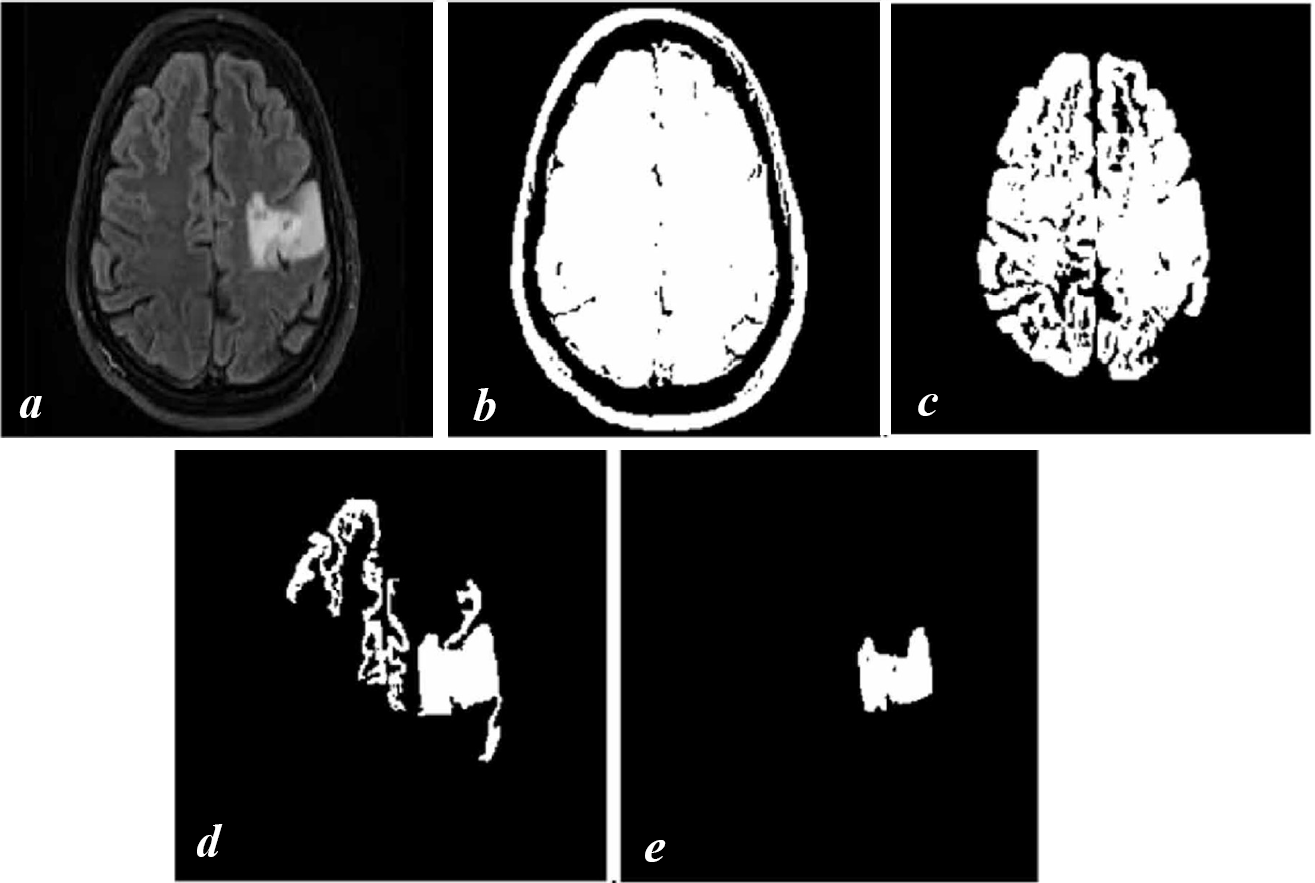
\includegraphics[width=0.8\columnwidth]{figures/Fig28.png}
	\caption{Example of the segmentation for different mean of BCET: a) original image, b) BCET 120, c) BCET 100, d) BCET 80, e) BCET 60}
	\label{fig28}
\end{figure}

\subsection{Adaptive Median Filtering (AMF)}
Image noise can be briefly defined as random variations in some of the pixel values of an image. We know filters are used to reduce the amount of noise present in an image. There are some outlier pixel values in images, due to these outlier cause disturbance (salt \& pepper) or also called as noise in images. Median filtering is excellent at reducing this type of noise. The filtering algorithm will scan the entire image, using a small matrix and recalculate the value of the center pixel by simply taking the median of all the values inside the matrix.

the median filter considers each pixel in the image in
turn and looks at its nearby neighbors to decide whether or not it is representative of its surroundings. Instead of simply replacing the pixel value with the mean of neighboring pixel values, it replaces it with the median of those values. The median is calculated by first sorting all the pixel values from the surrounding neighborhood into numerical order and then replacing the pixel being considered with the middle pixel value. The following example should clear the concept.

\begin{center}
	\[
	\textit{current value} =  
	\begin{bmatrix}
		19 & 12 & 38 \\
		42 & \textcolor{blue}{11} & 9 \\
		27 & 40 & 33
	\end{bmatrix}
	\]
	\textbf{Sort}: 9 , 11 , 12 , 19 , 27 , 33 , 38 , 40 , 42
	
	\textbf{Median}: 27
	\[
	\textit{after apply filter} =  
	\begin{bmatrix}
		19 & 12 & 38 \\
		42 & \textcolor{blue}{27} & 9 \\
		27 & 40 & 33
	\end{bmatrix}
	\]
\end{center}

The Adaptive Median Filter performs spatial processing to determine which
pixels in an image have been affected by impulse noise. The Adaptive Median Filter classifies pixels as noise by comparing each pixel in the image to its surrounding neighbor pixels. The size of the neighborhood is adjustable, as well as the threshold for the comparison. A pixel that is different from most of its neighbors, as well as being not structurally aligned with those pixels to which it is similar, is labeled as impulse noise. These noise pixels are then replaced by the
median pixel value of the pixels in the neighborhood that have passed the noise labeling test. 

The Adaptive Median Filter needs the following parameters:

\begin{itemize}
	\item \textbf{$S_{xy}$}: the support of the filter centered at (x, y)
	\item \textbf{$Z_{min}$}: minimum gray level value in $S_{xy}$
	\item \textbf{$Z_{max}$}: maximum gray level value in $S_{xy}$
	\item \textbf{$Z_{med}$}: median of gray levels in $S_{xy}$
	\item \textbf{$Z_{xy}$}: gray level at coordinates (x, y)
	\item \textbf{$S_{max}$}: maximum allowed size of $S_{xy}$
\end{itemize}

AMF uses the following algorithm (Algorithm \ref{Algo2}):

\begin{algorithm}[t]
	\caption{Adaptive Median Filter}
	\label{Algo2}
	\begin{spacing}{1.5}
		\begin{algorithmic}[1]
			\State \textbf{Level A:}
			\State A1 = $Z_{med}$ - $Z_{min}$
			\State A2 = $Z_{med}$ - $Z_{max}$
			\If{A1 > 0 AND A2 < 0}
			\State go to \textbf{level B}
			\Else
			\State increase the window size
			\If{window size < $S_{max}$}
			\State repeat level A
			\Else 
			\State output $Z_{xy}$
			\EndIf
			\EndIf
			\State \textbf{Level B:}
			\State B1 =  $Z_{xy}$ -  $Z_{min}$
			\State B2 =  $Z_{xy}$ -  $Z_{max}$
			\If{B1 > 0 AND B2 < 0}
			\State output $Z_{xy}$
			\Else
			\State output $Z_{med}$
			\EndIf
		\end{algorithmic}
	\end{spacing}
\end{algorithm}

\vspace{4cm}

\textbf{Level A} determines if the output of the filter $Z_{med}$ is an impulse or not(black or white). If it is not an impulse we go to \textbf{level B}. On the other hand, if it is an impulse, the window size is increased until it reaches the maximum window size or $Z_{med}$ is not an impulse. 

\textbf{level B} determines if the pixel value at (x, y), that is $Z_{xy}$, is an impulse or not. If it is not an impulse, the algorithm output wont change current $Z_{xy}$. But, if it is an impulse the algorithm output will be  $Z_{med}$. 

\subsection{Otsu’s Thresholding}

Converting a grayscale image to monochrome is a common image
processing task. Otsu's method, named after its inventor Nobuyuki Otsu, is one of many binarization algorithms, it uses data-driven approach which can adaptively find the optimal threshold to distinguish two-class data, by going through all possible threshold values (from 0 to 255), it can find the optimal threshold value of input image. This method can be applied in image segmentation and image binarization, in the current project the use was for image binarization.

Threshold is a value between 0 to 255. For example, if we set threshold value T = 128, then the image is separated into two classes, which are Class 1 (pixel value<= 128) and Class 2 (pixel value> 128) We can say that these two classes represent background and foreground of the input image, respectively.

\subsection{Canny Edge Detection}
In the final step of the algorithm, the 2 segmented images resulted from the segmentation process are combined using opencv \textbf{addWeighted} method by providing desired weights, the tumor being weighted more. This combined image is provided as an argument for the canny edge detection, the method highlights the tumor region and results with detected tumor output image.
There are many other methods which can be used for contour extraction such as Roberts, Prewitt, Sobel, and more complex ones like LoG but we used as a reference shown Canny method to be effective for contour extraction.

\subsection{Architecture of the system}
Figure \ref{fig29} illustrates the architecture of the system.

\newpage
\begin{figure}[H]
	%\resizebox{\linewidth}{!}{
	\centering 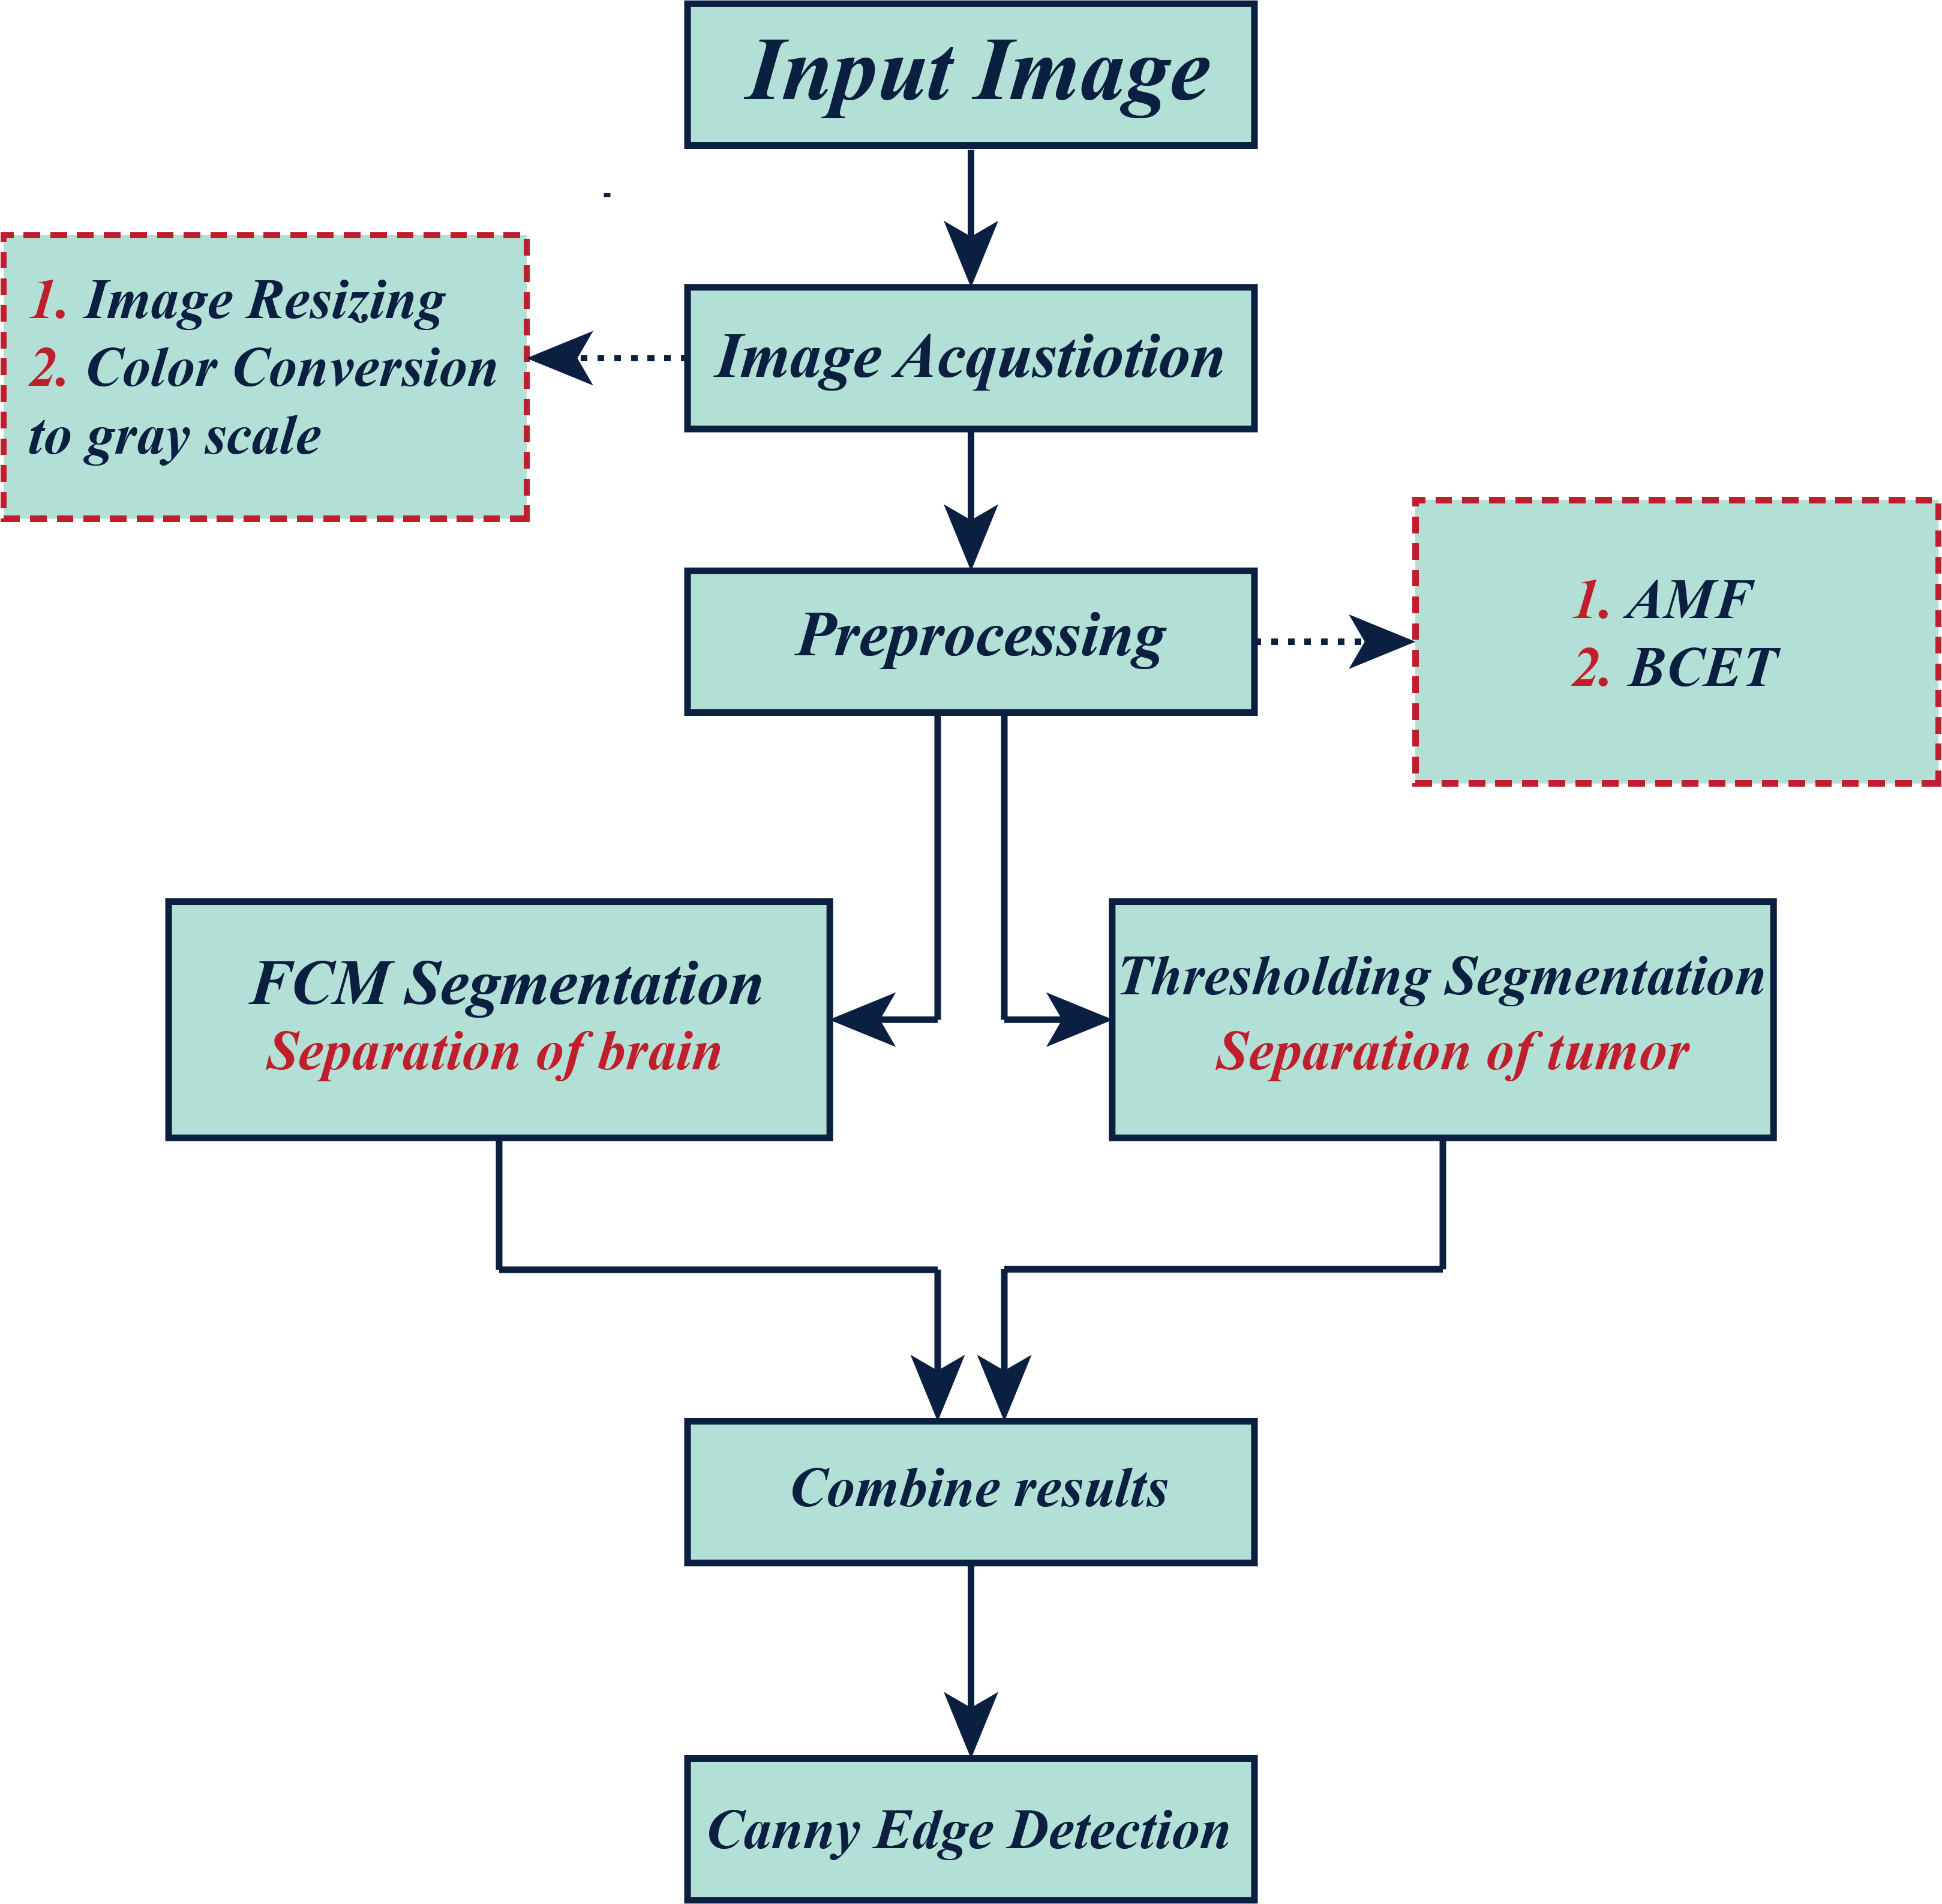
\includegraphics[width=1\columnwidth]{figures/Fig29.png}
	\caption{Architecture of the system}
	\label{fig29}
\end{figure}

\subsection{Implementation}

\begin{tcolorbox}[breakable, size=fbox, boxrule=1pt, pad at break*=1mm,colback=cellbackground, colframe=cellborder]
	\prompt{In}{incolor}{ }{\boxspacing}
	\begin{Verbatim}[commandchars=\\\{\}]
\PY{k+kn}{import} \PY{n+nn}{sys}
\PY{k+kn}{import} \PY{n+nn}{os}
\PY{k+kn}{from} \PY{n+nn}{time} \PY{k+kn}{import} \PY{n}{time}
\PY{k+kn}{import} \PY{n+nn}{cv2}
\PY{k+kn}{import} \PY{n+nn}{numpy} \PY{k}{as} \PY{n+nn}{np}
\PY{k+kn}{import} \PY{n+nn}{matplotlib}\PY{n+nn}{.}\PY{n+nn}{pyplot} \PY{k}{as} \PY{n+nn}{plt}
\PY{k+kn}{import} \PY{n+nn}{skfuzzy} \PY{k}{as} \PY{n+nn}{fuzz}
	\end{Verbatim}
\end{tcolorbox}

\begin{tcolorbox}[breakable, size=fbox, boxrule=1pt, pad at break*=1mm,colback=cellbackground, colframe=cellborder]
	\prompt{In}{incolor}{ }{\boxspacing}
	\begin{Verbatim}[commandchars=\\\{\}]
\PY{k}{def} \PY{n+nf}{AdaptiveMedianFilter}\PY{p}{(}\PY{n}{grayimage}\PY{p}{)}\PY{p}{:}
    \PY{k}{try}\PY{p}{:}
        \PY{n}{img\PYZus{}out} \PY{o}{=} \PY{n}{grayimage}\PY{o}{.}\PY{n}{copy}\PY{p}{(}\PY{p}{)}
        \PY{n}{height} \PY{o}{=} \PY{n}{grayimage}\PY{o}{.}\PY{n}{shape}\PY{p}{[}\PY{l+m+mi}{0}\PY{p}{]}
        \PY{n}{width} \PY{o}{=} \PY{n}{grayimage}\PY{o}{.}\PY{n}{shape}\PY{p}{[}\PY{l+m+mi}{1}\PY{p}{]}
        \PY{k}{for} \PY{n}{i} \PY{o+ow}{in} \PY{n}{np}\PY{o}{.}\PY{n}{arange}\PY{p}{(}\PY{l+m+mi}{6}\PY{p}{,} \PY{n}{height} \PY{o}{\PYZhy{}} \PY{l+m+mi}{5}\PY{p}{)}\PY{p}{:}
            \PY{k}{for} \PY{n}{j} \PY{o+ow}{in} \PY{n}{np}\PY{o}{.}\PY{n}{arange}\PY{p}{(}\PY{l+m+mi}{6}\PY{p}{,} \PY{n}{width} \PY{o}{\PYZhy{}} \PY{l+m+mi}{5}\PY{p}{)}\PY{p}{:}
                \PY{n}{neighbors} \PY{o}{=} \PY{p}{[}\PY{p}{]}
		
                \PY{k}{for} \PY{n}{k} \PY{o+ow}{in} \PY{n}{np}\PY{o}{.}\PY{n}{arange}\PY{p}{(}\PY{o}{\PYZhy{}}\PY{l+m+mi}{6}\PY{p}{,} \PY{l+m+mi}{6}\PY{p}{)}\PY{p}{:}
                    \PY{k}{for} \PY{n}{l} \PY{o+ow}{in} \PY{n}{np}\PY{o}{.}\PY{n}{arange}\PY{p}{(}\PY{o}{\PYZhy{}}\PY{l+m+mi}{6}\PY{p}{,} \PY{l+m+mi}{6}\PY{p}{)}\PY{p}{:}
                        \PY{n}{a} \PY{o}{=} \PY{n}{grayimage}\PY{o}{.}\PY{n}{item}\PY{p}{(}\PY{n}{i} \PY{o}{+} \PY{n}{k}\PY{p}{,} \PY{n}{j} \PY{o}{+} \PY{n}{l}\PY{p}{)}
                        \PY{n}{neighbors}\PY{o}{.}\PY{n}{append}\PY{p}{(}\PY{n}{a}\PY{p}{)}
        \PY{n}{neighbors}\PY{o}{.}\PY{n}{sort}\PY{p}{(}\PY{p}{)}
        \PY{n}{median} \PY{o}{=} \PY{n}{neighbors}\PY{p}{[}\PY{l+m+mi}{30}\PY{p}{]}
        \PY{n}{b} \PY{o}{=} \PY{n}{median}
        \PY{n}{img\PYZus{}out}\PY{o}{.}\PY{n}{itemset}\PY{p}{(}\PY{p}{(}\PY{n}{i}\PY{p}{,} \PY{n}{j}\PY{p}{)}\PY{p}{,} \PY{n}{b}\PY{p}{)}
		
    \PY{k}{except} \PY{n+ne}{Exception} \PY{k}{as} \PY{n}{e}\PY{p}{:}
        \PY{n+nb}{print}\PY{p}{(}\PY{l+s+s2}{\PYZdq{}}\PY{l+s+s2}{Error=}\PY{l+s+s2}{\PYZdq{}} \PY{o}{+} \PY{n}{e}\PY{o}{.}\PY{n}{args}\PY{p}{[}\PY{l+m+mi}{0}\PY{p}{]}\PY{p}{)}
        \PY{n}{tb} \PY{o}{=} \PY{n}{sys}\PY{o}{.}\PY{n}{exc\PYZus{}info}\PY{p}{(}\PY{p}{)}\PY{p}{[}\PY{l+m+mi}{2}\PY{p}{]}
		\PY{n+nb}{print}\PY{p}{(}\PY{n}{tb}\PY{o}{.}\PY{n}{tb\PYZus{}lineno}\PY{p}{)}
		
    \PY{k}{return} \PY{n}{img\PYZus{}out}\PY{o}{.}\PY{n}{astype}\PY{p}{(}\PY{n}{np}\PY{o}{.}\PY{n}{uint8}\PY{p}{)}
	\end{Verbatim}
\end{tcolorbox}

\begin{tcolorbox}[breakable, size=fbox, boxrule=1pt, pad at break*=1mm,colback=cellbackground, colframe=cellborder]
	\prompt{In}{incolor}{ }{\boxspacing}
	\begin{Verbatim}[commandchars=\\\{\}]
\PY{k}{def} \PY{n+nf}{BalanceContrastEnhancementTechnique}\PY{p}{(}\PY{n}{gray\PYZus{}image}\PY{p}{)}\PY{p}{:}
    \PY{n}{x} \PY{o}{=} \PY{n}{im2double}\PY{p}{(}\PY{n}{gray\PYZus{}image}\PY{p}{)} \PY{c+c1}{\PYZsh{} INPUT IMAGE}
    \PY{n}{Lmin} \PY{o}{=} \PY{n}{np}\PY{o}{.}\PY{n}{min}\PY{p}{(}\PY{n}{x}\PY{o}{.}\PY{n}{ravel}\PY{p}{(}\PY{p}{)}\PY{p}{)} \PY{c+c1}{\PYZsh{} MINIMUM OF INPUT IMAGE}
    \PY{n}{Lmax} \PY{o}{=}\PY{n}{np}\PY{o}{.}\PY{n}{max}\PY{p}{(}\PY{n}{x}\PY{o}{.}\PY{n}{ravel}\PY{p}{(}\PY{p}{)}\PY{p}{)} \PY{c+c1}{\PYZsh{} MAXIMUM OF INPUT IMAGE}
    \PY{n}{Lmean} \PY{o}{=} \PY{n}{np}\PY{o}{.}\PY{n}{mean}\PY{p}{(}\PY{n}{x}\PY{p}{)} \PY{c+c1}{\PYZsh{} MEAN OF INPUT IMAGE}
    \PY{n}{LMssum} \PY{o}{=} \PY{n}{np}\PY{o}{.}\PY{n}{mean}\PY{p}{(}\PY{n+nb}{pow}\PY{p}{(}\PY{n}{x}\PY{p}{,}\PY{l+m+mi}{2}\PY{p}{)}\PY{p}{)} \PY{c+c1}{\PYZsh{} MEAN SQUARE SUM OF INPUT IMAGE}

    \PY{n}{Gmin} \PY{o}{=} \PY{l+m+mi}{0} \PY{c+c1}{\PYZsh{} MINIMUM OF OUTPUT IMAGE}
    \PY{n}{Gmax} \PY{o}{=} \PY{l+m+mi}{255} \PY{c+c1}{\PYZsh{} MAXIMUM OF OUTPUT IMAGE}
    \PY{n}{Gmean} \PY{o}{=}\PY{l+m+mi}{85} \PY{c+c1}{\PYZsh{} MEAN OF OUTPUT IMAGE 80 (Recomended)}

    \PY{n}{bnum} \PY{o}{=} \PY{n+nb}{pow}\PY{p}{(}\PY{n}{Lmax}\PY{p}{,}\PY{l+m+mi}{2}\PY{p}{)} \PY{o}{*} \PY{p}{(}\PY{n}{Gmean} \PY{o}{\PYZhy{}} \PY{n}{Gmin}\PY{p}{)} \PY{o}{\PYZhy{}} \PY{n}{LMssum} \PY{o}{*} \PY{p}{(}\PY{n}{Gmax} \PY{o}{\PYZhy{}} \PY{n}{Gmin}\PY{p}{)} \PY{o}{+}
    \PY{n+nb}{pow}\PY{p}{(}\PY{n}{Lmin}\PY{p}{,}\PY{l+m+mi}{2}\PY{p}{)} \PY{o}{*} \PY{p}{(}\PY{n}{Gmax} \PY{o}{\PYZhy{}} \PY{n}{Gmean}\PY{p}{)}
    \PY{n}{bden} \PY{o}{=} \PY{l+m+mi}{2} \PY{o}{*} \PY{p}{(}\PY{n}{Lmax} \PY{o}{*} \PY{p}{(}\PY{n}{Gmean} \PY{o}{\PYZhy{}} \PY{n}{Gmin}\PY{p}{)} \PY{o}{\PYZhy{}} \PY{n}{Lmean} \PY{o}{*} \PY{p}{(}\PY{n}{Gmax} \PY{o}{\PYZhy{}} \PY{n}{Gmin}\PY{p}{)} \PY{o}{+} \PY{n}{Lmin} \PY{o}{*}
    \PY{p}{(}\PY{n}{Gmax} \PY{o}{\PYZhy{}} \PY{n}{Gmean}\PY{p}{)}\PY{p}{)}

    \PY{n}{b} \PY{o}{=} \PY{n}{bnum} \PY{o}{/} \PY{n}{bden}
    \PY{n}{a} \PY{o}{=} \PY{p}{(}\PY{n}{Gmax} \PY{o}{\PYZhy{}} \PY{n}{Gmin}\PY{p}{)} \PY{o}{/} \PY{p}{(}\PY{p}{(}\PY{n}{Lmax} \PY{o}{\PYZhy{}} \PY{n}{Lmin}\PY{p}{)} \PY{o}{*} \PY{p}{(}\PY{n}{Lmax} \PY{o}{+} \PY{n}{Lmin} \PY{o}{\PYZhy{}} \PY{l+m+mi}{2} \PY{o}{*} \PY{n}{b}\PY{p}{)}\PY{p}{)}
    \PY{n}{c} \PY{o}{=} \PY{n}{Gmin} \PY{o}{\PYZhy{}} \PY{n}{a} \PY{o}{*} \PY{n+nb}{pow}\PY{p}{(}\PY{p}{(}\PY{n}{Lmin} \PY{o}{\PYZhy{}} \PY{n}{b}\PY{p}{)}\PY{p}{,} \PY{l+m+mi}{2}\PY{p}{)}
    \PY{n}{y} \PY{o}{=} \PY{n}{a} \PY{o}{*}\PY{n+nb}{pow}\PY{p}{(}\PY{p}{(}\PY{n}{x} \PY{o}{\PYZhy{}} \PY{n}{b}\PY{p}{)}\PY{p}{,}\PY{l+m+mi}{2}\PY{p}{)}\PY{o}{+} \PY{n}{c} \PY{c+c1}{\PYZsh{} PARABOLIC FUNCTION}
    \PY{n}{y} \PY{o}{=} \PY{n}{y}\PY{o}{.}\PY{n}{astype}\PY{p}{(}\PY{n}{np}\PY{o}{.}\PY{n}{uint8}\PY{p}{)}

    \PY{k}{return} \PY{n}{y}
	\end{Verbatim}
\end{tcolorbox}

\begin{tcolorbox}[breakable, size=fbox, boxrule=1pt, pad at break*=1mm,colback=cellbackground, colframe=cellborder]
	\prompt{In}{incolor}{ }{\boxspacing}
	\begin{Verbatim}[commandchars=\\\{\}]
\PY{k}{def} \PY{n+nf}{im2double}\PY{p}{(}\PY{n}{im}\PY{p}{)}\PY{p}{:}
    \PY{n}{min\PYZus{}val} \PY{o}{=} \PY{n}{np}\PY{o}{.}\PY{n}{min}\PY{p}{(}\PY{n}{im}\PY{o}{.}\PY{n}{ravel}\PY{p}{(}\PY{p}{)}\PY{p}{)}
    \PY{n}{max\PYZus{}val} \PY{o}{=} \PY{n}{np}\PY{o}{.}\PY{n}{max}\PY{p}{(}\PY{n}{im}\PY{o}{.}\PY{n}{ravel}\PY{p}{(}\PY{p}{)}\PY{p}{)}
    \PY{n}{out} \PY{o}{=} \PY{p}{(}\PY{n}{im}\PY{o}{.}\PY{n}{astype}\PY{p}{(}\PY{l+s+s1}{\PYZsq{}}\PY{l+s+s1}{float}\PY{l+s+s1}{\PYZsq{}}\PY{p}{)} \PY{o}{\PYZhy{}} \PY{n}{min\PYZus{}val}\PY{p}{)} \PY{o}{/} \PY{p}{(}\PY{n}{max\PYZus{}val} \PY{o}{\PYZhy{}} \PY{n}{min\PYZus{}val}\PY{p}{)}
    \PY{k}{return} \PY{n}{out}
	\end{Verbatim}
\end{tcolorbox}

NumPy python package is used to calculate the min,max,mean of the input
image by converting the given image pixel array to double precession and
flattening out the array using NumPy ravel function and applying desired
min,max functions existing in NumPy package. The resultant `y' is the
new enhanced/stretched contrast image, this image is used in further
processing for thresholding and contour extraction.

\begin{tcolorbox}[breakable, size=fbox, boxrule=1pt, pad at break*=1mm,colback=cellbackground, colframe=cellborder]
	\prompt{In}{incolor}{ }{\boxspacing}
	\begin{Verbatim}[commandchars=\\\{\}]
\PY{k}{def} \PY{n+nf}{FCM}\PY{p}{(}\PY{n}{image\PYZus{}bcet}\PY{p}{)}\PY{p}{:}
    \PY{n}{list\PYZus{}img} \PY{o}{=} \PY{p}{[}\PY{p}{]}
    \PY{n}{img} \PY{o}{=}\PY{n}{cv2}\PY{o}{.}\PY{n}{imread}\PY{p}{(}\PY{l+s+s2}{\PYZdq{}}\PY{l+s+s2}{C:/Users/Poorya/Desktop/}\PY{l+s+s2}{\PYZdq{}}\PY{o}{+}\PY{n+nb}{str}\PY{p}{(}\PY{n}{image\PYZus{}bcet}\PY{p}{)}\PY{p}{)}

    \PY{n}{rgb\PYZus{}img} \PY{o}{=} \PY{n}{img}\PY{o}{.}\PY{n}{reshape}\PY{p}{(}\PY{p}{(}\PY{n}{img}\PY{o}{.}\PY{n}{shape}\PY{p}{[}\PY{l+m+mi}{0}\PY{p}{]} \PY{o}{*} \PY{n}{img}\PY{o}{.}\PY{n}{shape}\PY{p}{[}\PY{l+m+mi}{1}\PY{p}{]}\PY{p}{,} \PY{l+m+mi}{3}\PY{p}{)}\PY{p}{)}
    \PY{n}{list\PYZus{}img}\PY{o}{.}\PY{n}{append}\PY{p}{(}\PY{n}{rgb\PYZus{}img}\PY{p}{)}
    \PY{n}{n\PYZus{}data} \PY{o}{=} \PY{n+nb}{len}\PY{p}{(}\PY{n}{list\PYZus{}img}\PY{p}{)}
    \PY{n}{clusters} \PY{o}{=} \PY{p}{[}\PY{l+m+mi}{2}\PY{p}{]}

    \PY{k}{for} \PY{n}{index}\PY{p}{,} \PY{n}{rgb\PYZus{}img} \PY{o+ow}{in} \PY{n+nb}{enumerate}\PY{p}{(}\PY{n}{list\PYZus{}img}\PY{p}{)}\PY{p}{:}
        \PY{n}{img} \PY{o}{=} \PY{n}{np}\PY{o}{.}\PY{n}{reshape}\PY{p}{(}\PY{n}{rgb\PYZus{}img}\PY{p}{,} \PY{p}{(}\PY{l+m+mi}{256}\PY{p}{,} \PY{l+m+mi}{256}\PY{p}{,} \PY{l+m+mi}{3}\PY{p}{)}\PY{p}{)}\PY{o}{.}\PY{n}{astype}\PY{p}{(}\PY{n}{np}\PY{o}{.}\PY{n}{uint8}\PY{p}{)}
        \PY{n}{shape} \PY{o}{=} \PY{n}{np}\PY{o}{.}\PY{n}{shape}\PY{p}{(}\PY{n}{img}\PY{p}{)}
        \PY{c+c1}{\PYZsh{} looping every cluster}
        \PY{k}{for} \PY{n}{i}\PY{p}{,} \PY{n}{cluster} \PY{o+ow}{in} \PY{n+nb}{enumerate}\PY{p}{(}\PY{n}{clusters}\PY{p}{)}\PY{p}{:}
            \PY{c+c1}{\PYZsh{} Fuzzy C Means}
            \PY{n}{new\PYZus{}time} \PY{o}{=} \PY{n}{time}\PY{p}{(}\PY{p}{)}

            \PY{n}{cntr}\PY{p}{,} \PY{n}{u}\PY{p}{,} \PY{n}{u0}\PY{p}{,} \PY{n}{d}\PY{p}{,} \PY{n}{jm}\PY{p}{,} \PY{n}{p}\PY{p}{,} \PY{n}{fpc} \PY{o}{=} \PY{n}{fuzz}\PY{o}{.}\PY{n}{cluster}\PY{o}{.}\PY{n}{cmeans}\PY{p}{(}\PY{n}{rgb\PYZus{}img}\PY{o}{.}\PY{n}{T}\PY{p}{,}
            \PY{n}{cluster}\PY{p}{,} \PY{l+m+mi}{2}\PY{p}{,} \PY{n}{error}\PY{o}{=}\PY{l+m+mf}{0.005}\PY{p}{,} \PY{n}{maxiter}\PY{o}{=}\PY{l+m+mi}{1000}\PY{p}{,} \PY{n}{init}\PY{o}{=}\PY{k+kc}{None}\PY{p}{,} \PY{n}{seed}\PY{o}{=}\PY{l+m+mi}{42}\PY{p}{)}
            \PY{n}{new\PYZus{}img} \PY{o}{=} \PY{n}{change\PYZus{}color\PYZus{}fuzzycmeans}\PY{p}{(}\PY{n}{u}\PY{p}{,} \PY{n}{cntr}\PY{p}{)}
            \PY{n}{fuzzy\PYZus{}img} \PY{o}{=} \PY{n}{np}\PY{o}{.}\PY{n}{reshape}\PY{p}{(}\PY{n}{new\PYZus{}img}\PY{p}{,} \PY{n}{shape}\PY{p}{)}\PY{o}{.}\PY{n}{astype}\PY{p}{(}\PY{n}{np}\PY{o}{.}\PY{n}{uint8}\PY{p}{)}
            \PY{n}{ret}\PY{p}{,} \PY{n}{seg\PYZus{}img} \PY{o}{=} \PY{n}{cv2}\PY{o}{.}\PY{n}{threshold}\PY{p}{(}\PY{n}{fuzzy\PYZus{}img}\PY{p}{,}\PY{n}{np}\PY{o}{.}\PY{n}{max}\PY{p}{(}\PY{n}{fuzzy\PYZus{}img}\PY{p}{)} \PY{o}{\PYZhy{}}
            \PY{l+m+mi}{1}\PY{p}{,}\PY{l+m+mi}{255}\PY{p}{,}\PY{n}{cv2}\PY{o}{.}\PY{n}{THRESH\PYZus{}BINARY}\PY{p}{)}

            \PY{n}{seg\PYZus{}img\PYZus{}1d} \PY{o}{=} \PY{n}{seg\PYZus{}img}\PY{p}{[}\PY{p}{:}\PY{p}{,} \PY{p}{:}\PY{p}{,} \PY{l+m+mi}{1}\PY{p}{]}
            \PY{n}{bwfim1} \PY{o}{=} \PY{n}{bwareaopen}\PY{p}{(}\PY{n}{seg\PYZus{}img\PYZus{}1d}\PY{p}{,} \PY{l+m+mi}{500}\PY{p}{)}
            \PY{n}{bwfim2} \PY{o}{=} \PY{n}{imclearborder}\PY{p}{(}\PY{n}{bwfim1}\PY{p}{)}

            \PY{n}{cv2}\PY{o}{.}\PY{n}{imwrite}\PY{p}{(}\PY{l+s+s1}{\PYZsq{}}\PY{l+s+s1}{C:/Users/Poorya/Desktop/border.jpg}\PY{l+s+s1}{\PYZsq{}}\PY{p}{,} \PY{n}{bwfim2}\PY{p}{)}


            \PY{n}{bwfim3} \PY{o}{=} \PY{n}{imfill}\PY{p}{(}\PY{n}{bwfim2}\PY{p}{)}    

            \PY{n}{cv2}\PY{o}{.}\PY{n}{imwrite}\PY{p}{(}\PY{l+s+s1}{\PYZsq{}}\PY{l+s+s1}{C:/Users/Poorya/Desktop/FCM.jpg}\PY{l+s+s1}{\PYZsq{}}\PY{p}{,} \PY{n}{bwfim3}\PY{p}{)}
    \PY{k}{return} \PY{n}{bwfim3}
	\end{Verbatim}
\end{tcolorbox}

\begin{tcolorbox}[breakable, size=fbox, boxrule=1pt, pad at break*=1mm,colback=cellbackground, colframe=cellborder]
	\prompt{In}{incolor}{ }{\boxspacing}
	\begin{Verbatim}[commandchars=\\\{\}]
\PY{k}{def} \PY{n+nf}{change\PYZus{}color\PYZus{}fuzzycmeans}\PY{p}{(}\PY{n}{cluster\PYZus{}membership}\PY{p}{,} \PY{n}{clusters}\PY{p}{)}\PY{p}{:}
    \PY{n}{img} \PY{o}{=} \PY{p}{[}\PY{p}{]}
    \PY{k}{for} \PY{n}{pix} \PY{o+ow}{in} \PY{n}{cluster\PYZus{}membership}\PY{o}{.}\PY{n}{T}\PY{p}{:}
        \PY{n}{img}\PY{o}{.}\PY{n}{append}\PY{p}{(}\PY{n}{clusters}\PY{p}{[}\PY{n}{np}\PY{o}{.}\PY{n}{argmax}\PY{p}{(}\PY{n}{pix}\PY{p}{)}\PY{p}{]}\PY{p}{)}
    \PY{k}{return} \PY{n}{img}
	\end{Verbatim}
\end{tcolorbox}

\begin{tcolorbox}[breakable, size=fbox, boxrule=1pt, pad at break*=1mm,colback=cellbackground, colframe=cellborder]
	\prompt{In}{incolor}{ }{\boxspacing}
	\begin{Verbatim}[commandchars=\\\{\}]
\PY{k}{def} \PY{n+nf}{imfill}\PY{p}{(}\PY{n}{im\PYZus{}th}\PY{p}{)}\PY{p}{:}
    \PY{n}{im\PYZus{}floodfill} \PY{o}{=} \PY{n}{im\PYZus{}th}\PY{o}{.}\PY{n}{copy}\PY{p}{(}\PY{p}{)}
    \PY{c+c1}{\PYZsh{} Mask used to flood filling.}
    \PY{c+c1}{\PYZsh{} Notice the size needs to be 2 pixels than the image.}
    \PY{n}{h}\PY{p}{,} \PY{n}{w} \PY{o}{=} \PY{n}{im\PYZus{}th}\PY{o}{.}\PY{n}{shape}\PY{p}{[}\PY{p}{:}\PY{l+m+mi}{2}\PY{p}{]}
    \PY{n}{mask} \PY{o}{=} \PY{n}{np}\PY{o}{.}\PY{n}{zeros}\PY{p}{(}\PY{p}{(}\PY{n}{h} \PY{o}{+} \PY{l+m+mi}{2}\PY{p}{,} \PY{n}{w} \PY{o}{+} \PY{l+m+mi}{2}\PY{p}{)}\PY{p}{,} \PY{n}{np}\PY{o}{.}\PY{n}{uint8}\PY{p}{)}
    \PY{c+c1}{\PYZsh{} Floodfill from point (0, 0)}
    \PY{n}{cv2}\PY{o}{.}\PY{n}{floodFill}\PY{p}{(}\PY{n}{im\PYZus{}floodfill}\PY{p}{,} \PY{n}{mask}\PY{p}{,} \PY{p}{(}\PY{l+m+mi}{0}\PY{p}{,} \PY{l+m+mi}{0}\PY{p}{)}\PY{p}{,} \PY{l+m+mi}{255}\PY{p}{)}\PY{p}{;}
    \PY{c+c1}{\PYZsh{} Invert floodfilled image}
    \PY{n}{im\PYZus{}floodfill\PYZus{}inv} \PY{o}{=} \PY{n}{cv2}\PY{o}{.}\PY{n}{bitwise\PYZus{}not}\PY{p}{(}\PY{n}{im\PYZus{}floodfill}\PY{p}{)}
    \PY{c+c1}{\PYZsh{} Combine the two images to get the foreground.}
    \PY{n}{im\PYZus{}out} \PY{o}{=} \PY{n}{im\PYZus{}th} \PY{o}{|} \PY{n}{im\PYZus{}floodfill\PYZus{}inv}
    \PY{k}{return} \PY{n}{im\PYZus{}out}
	\end{Verbatim}
\end{tcolorbox}

 After clustering, the cluster centers are passed to custom function and
a new image is constructed according to the cluster membership.
Thresholding is performed on this image using opencv threshold method,
this is usually done for optimal contour extraction.

{Contours} can be explained simply as a curve joining all the continuous
points (along the boundary), having same color or intensity. The
contours are a useful tool for shape analysis and object detection and
recognition.Here they suggest performing thresholding before contour
extraction. The contour extraction is applied at 2 different stages:

\begin{tcolorbox}[breakable, size=fbox, boxrule=1pt, pad at break*=1mm,colback=cellbackground, colframe=cellborder]
	\prompt{In}{incolor}{ }{\boxspacing}
	\begin{Verbatim}[commandchars=\\\{\}]
\PY{k}{def} \PY{n+nf}{bwareaopen}\PY{p}{(}\PY{n}{imgBW}\PY{p}{,} \PY{n}{areaPixels}\PY{p}{)}\PY{p}{:}
    \PY{c+c1}{\PYZsh{} Given a black and white image, first find all of its contours}
    \PY{n}{imgBWcopy} \PY{o}{=} \PY{n}{imgBW}\PY{o}{.}\PY{n}{copy}\PY{p}{(}\PY{p}{)}
    \PY{n}{contours}\PY{p}{,} \PY{n}{hierarchy} \PY{o}{=} \PY{n}{cv2}\PY{o}{.}\PY{n}{findContours}\PY{p}{(}\PY{n}{imgBWcopy}\PY{o}{.}\PY{n}{copy}\PY{p}{(}\PY{p}{)}\PY{p}{,} \PY{n}{cv2}\PY{o}{.}\PY{n}{RETR\PYZus{}LIST}\PY{p}{,}\PY{n}{cv2}\PY{o}{.}\PY{n}{CHAIN\PYZus{}APPROX\PYZus{}SIMPLE}\PY{p}{)}
    \PY{c+c1}{\PYZsh{} For each contour, determine its total occupying area}
    \PY{k}{for} \PY{n}{idx} \PY{o+ow}{in} \PY{n}{np}\PY{o}{.}\PY{n}{arange}\PY{p}{(}\PY{n+nb}{len}\PY{p}{(}\PY{n}{contours}\PY{p}{)}\PY{p}{)}\PY{p}{:}
        \PY{n}{area} \PY{o}{=} \PY{n}{cv2}\PY{o}{.}\PY{n}{contourArea}\PY{p}{(}\PY{n}{contours}\PY{p}{[}\PY{n}{idx}\PY{p}{]}\PY{p}{)}
        \PY{k}{if} \PY{p}{(}\PY{n}{area} \PY{o}{\PYZgt{}}\PY{o}{=} \PY{l+m+mi}{0} \PY{o+ow}{and} \PY{n}{area} \PY{o}{\PYZlt{}}\PY{o}{=} \PY{n}{areaPixels}\PY{p}{)}\PY{p}{:}
            \PY{n}{cv2}\PY{o}{.}\PY{n}{drawContours}\PY{p}{(}\PY{n}{imgBWcopy}\PY{p}{,} \PY{n}{contours}\PY{p}{,} \PY{n}{idx}\PY{p}{,} \PY{p}{(}\PY{l+m+mi}{0}\PY{p}{,} \PY{l+m+mi}{0}\PY{p}{,} \PY{l+m+mi}{0}\PY{p}{)}\PY{p}{,} \PY{o}{\PYZhy{}}\PY{l+m+mi}{1}\PY{p}{)}

    \PY{k}{return} \PY{n}{imgBWcopy}
	\end{Verbatim}
\end{tcolorbox}

 The above function determines the total occupying area of each contour
and on comparing with the fixed value of area pixels- set to 500, this
is value is used to preserve and draw the contours which ranges in the
specific area. All the extracted contours which fall in the range are
redrawn using opencv drawcontours method.

The next step is a selection the boundary pixels (edge pixels). A pixel
is considered as boundary pixel if the magnitude of the gradient of this
pixel is greater than that of two neighbors in the direction of the
gradient In the below method, each contour row and column pixel is
evaluated, the row and column check conditions are used to determine the
border of the brain and hence appending to a new list of contours, this
list is redrawn using drawContours method. This image is the final FCM
segmented image.

\begin{tcolorbox}[breakable, size=fbox, boxrule=1pt, pad at break*=1mm,colback=cellbackground, colframe=cellborder]
	\prompt{In}{incolor}{ }{\boxspacing}
	\begin{Verbatim}[commandchars=\\\{\}]
\PY{k}{def} \PY{n+nf}{imclearborder}\PY{p}{(}\PY{n}{imgBW}\PY{p}{)}\PY{p}{:}
    \PY{c+c1}{\PYZsh{} Given a black and white image, first find all of its contours}
    \PY{n}{radius} \PY{o}{=} \PY{l+m+mi}{2}
    \PY{n}{imgBWcopy} \PY{o}{=} \PY{n}{imgBW}\PY{o}{.}\PY{n}{copy}\PY{p}{(}\PY{p}{)}

    \PY{n}{contours}\PY{p}{,} \PY{n}{hierarchy} \PY{o}{=} \PY{n}{cv2}\PY{o}{.}\PY{n}{findContours}\PY{p}{(}\PY{n}{imgBWcopy}\PY{o}{.}\PY{n}{copy}\PY{p}{(}\PY{p}{)}\PY{p}{,} \PY{n}{cv2}\PY{o}{.}\PY{n}{RETR\PYZus{}LIST}\PY{p}{,}\PY{n}{cv2}\PY{o}{.}\PY{n}{CHAIN\PYZus{}APPROX\PYZus{}SIMPLE}\PY{p}{)}

    \PY{c+c1}{\PYZsh{} Get dimensions of image}
    \PY{n}{imgRows} \PY{o}{=} \PY{n}{imgBW}\PY{o}{.}\PY{n}{shape}\PY{p}{[}\PY{l+m+mi}{0}\PY{p}{]}
    \PY{n}{imgCols} \PY{o}{=} \PY{n}{imgBW}\PY{o}{.}\PY{n}{shape}\PY{p}{[}\PY{l+m+mi}{1}\PY{p}{]}
    \PY{n}{contourList} \PY{o}{=} \PY{p}{[}\PY{p}{]} \PY{c+c1}{\PYZsh{} ID list of contours that touch the border}

    \PY{c+c1}{\PYZsh{} For each contour...}
    \PY{k}{for} \PY{n}{idx} \PY{o+ow}{in} \PY{n}{np}\PY{o}{.}\PY{n}{arange}\PY{p}{(}\PY{n+nb}{len}\PY{p}{(}\PY{n}{contours}\PY{p}{)}\PY{p}{)}\PY{p}{:}
        \PY{c+c1}{\PYZsh{} Get the i\PYZsq{}th contour}
        \PY{n}{cnt} \PY{o}{=} \PY{n}{contours}\PY{p}{[}\PY{n}{idx}\PY{p}{]}
        \PY{c+c1}{\PYZsh{} Look at each point in the contour}
        \PY{k}{for} \PY{n}{pt} \PY{o+ow}{in} \PY{n}{cnt}\PY{p}{:}
            \PY{n}{rowCnt} \PY{o}{=} \PY{n}{pt}\PY{p}{[}\PY{l+m+mi}{0}\PY{p}{]}\PY{p}{[}\PY{l+m+mi}{1}\PY{p}{]}
            \PY{n}{colCnt} \PY{o}{=} \PY{n}{pt}\PY{p}{[}\PY{l+m+mi}{0}\PY{p}{]}\PY{p}{[}\PY{l+m+mi}{0}\PY{p}{]}
            \PY{c+c1}{\PYZsh{} If this is within the radius of the border}
            \PY{c+c1}{\PYZsh{} this contour goes bye bye!}
            \PY{n}{check1} \PY{o}{=} \PY{p}{(}\PY{n}{rowCnt} \PY{o}{\PYZgt{}}\PY{o}{=} \PY{l+m+mi}{0} \PY{o+ow}{and} \PY{n}{rowCnt} \PY{o}{\PYZlt{}} \PY{n}{radius}\PY{p}{)} \PY{o+ow}{or} \PY{p}{(}\PY{n}{rowCnt}
            \PY{o}{\PYZgt{}}\PY{o}{=} \PY{n}{imgRows} \PY{o}{\PYZhy{}} \PY{l+m+mi}{1} \PY{o}{\PYZhy{}} \PY{n}{radius} \PY{o+ow}{and} \PY{n}{rowCnt} \PY{o}{\PYZlt{}} \PY{n}{imgRows}\PY{p}{)}
            \PY{n}{check2} \PY{o}{=} \PY{p}{(}\PY{n}{colCnt} \PY{o}{\PYZgt{}}\PY{o}{=} \PY{l+m+mi}{0} \PY{o+ow}{and} \PY{n}{colCnt} \PY{o}{\PYZlt{}} \PY{n}{radius}\PY{p}{)} \PY{o+ow}{or} \PY{p}{(}\PY{n}{colCnt} \PY{o}{\PYZgt{}}\PY{o}{=}
            \PY{n}{imgCols} \PY{o}{\PYZhy{}} \PY{l+m+mi}{1} \PY{o}{\PYZhy{}} \PY{n}{radius} \PY{o+ow}{and} \PY{n}{colCnt} \PY{o}{\PYZlt{}} \PY{n}{imgCols}\PY{p}{)} 

            \PY{k}{if} \PY{n}{check1} \PY{o+ow}{or} \PY{n}{check2}\PY{p}{:}
                \PY{n}{contourList}\PY{o}{.}\PY{n}{append}\PY{p}{(}\PY{n}{idx}\PY{p}{)}
                \PY{k}{break}

        \PY{k}{for} \PY{n}{idx} \PY{o+ow}{in} \PY{n}{contourList}\PY{p}{:}
            \PY{n}{cv2}\PY{o}{.}\PY{n}{drawContours}\PY{p}{(}\PY{n}{imgBWcopy}\PY{p}{,} \PY{n}{contours}\PY{p}{,} \PY{n}{idx}\PY{p}{,} \PY{p}{(}\PY{l+m+mi}{0}\PY{p}{,} \PY{l+m+mi}{0}\PY{p}{,} \PY{l+m+mi}{0}\PY{p}{)}\PY{p}{,} \PY{o}{\PYZhy{}}\PY{l+m+mi}{1}\PY{p}{)}           
    \PY{k}{return} \PY{n}{imgBWcopy}
	\end{Verbatim}
\end{tcolorbox}

\begin{tcolorbox}[breakable, size=fbox, boxrule=1pt, pad at break*=1mm,colback=cellbackground, colframe=cellborder]
	\prompt{In}{incolor}{ }{\boxspacing}
	\begin{Verbatim}[commandchars=\\\{\}]
\PY{k}{def} \PY{n+nf}{Thresholding}\PY{p}{(}\PY{n}{image\PYZus{}bcet}\PY{p}{)}\PY{p}{:}
    \PY{n}{blur} \PY{o}{=} \PY{n}{cv2}\PY{o}{.}\PY{n}{GaussianBlur}\PY{p}{(}\PY{n}{image\PYZus{}bcet}\PY{p}{,}\PY{p}{(}\PY{l+m+mi}{5}\PY{p}{,}\PY{l+m+mi}{5}\PY{p}{)}\PY{p}{,}\PY{l+m+mi}{0}\PY{p}{)}
    \PY{n}{T}\PY{p}{,} \PY{n}{thresh\PYZus{}f} \PY{o}{=} \PY{n}{cv2}\PY{o}{.}\PY{n}{threshold}\PY{p}{(}\PY{n}{blur}\PY{p}{,}\PY{l+m+mi}{200}\PY{p}{,}\PY{l+m+mi}{255}\PY{p}{,}   \PY{n}{cv2}\PY{o}{.}\PY{n}{THRESH\PYZus{}BINARY}\PY{p}{)}
    \PY{k}{return} \PY{n}{thresh\PYZus{}f}
	\end{Verbatim}
\end{tcolorbox}

\begin{tcolorbox}[breakable, size=fbox, boxrule=1pt, pad at break*=1mm,colback=cellbackground, colframe=cellborder]
	\prompt{In}{incolor}{ }{\boxspacing}
	\begin{Verbatim}[commandchars=\\\{\}]
\PY{k}{def} \PY{n+nf}{segmentation}\PY{p}{(}\PY{n}{fcm\PYZus{}image}\PY{p}{,}\PY{n}{ths\PYZus{}image}\PY{p}{)}\PY{p}{:}
    \PY{n}{brain} \PY{o}{=} \PY{n}{fcm\PYZus{}image}
    \PY{n}{tumor} \PY{o}{=} \PY{n}{ths\PYZus{}image}
    \PY{n}{segimg} \PY{o}{=} \PY{n}{cv2}\PY{o}{.}\PY{n}{addWeighted}\PY{p}{(}\PY{n}{brain}\PY{p}{,} \PY{l+m+mf}{0.5}\PY{p}{,} \PY{n}{tumor}\PY{p}{,} \PY{l+m+mf}{0.7}\PY{p}{,} \PY{l+m+mi}{0}\PY{p}{)}
    \PY{k}{return} \PY{n}{segimg}
	\end{Verbatim}
\end{tcolorbox}

\begin{tcolorbox}[breakable, size=fbox, boxrule=1pt, pad at break*=1mm,colback=cellbackground, colframe=cellborder]
	\prompt{In}{incolor}{ }{\boxspacing}
	\begin{Verbatim}[commandchars=\\\{\}]
\PY{k}{def} \PY{n+nf}{dataanalysis}\PY{p}{(}\PY{n}{seg\PYZus{}img}\PY{p}{)}\PY{p}{:}
    \PY{k}{try}\PY{p}{:}
        \PY{n}{detected\PYZus{}edges} \PY{o}{=} \PY{n}{cv2}\PY{o}{.}\PY{n}{Canny}\PY{p}{(}\PY{n}{seg\PYZus{}img}\PY{p}{,} \PY{l+m+mi}{10}\PY{p}{,} \PY{l+m+mi}{10} \PY{o}{*} \PY{l+m+mi}{3}\PY{p}{,} \PY{l+m+mi}{5}\PY{p}{)}
        \PY{n}{colour} \PY{o}{=} \PY{n}{cv2}\PY{o}{.}\PY{n}{applyColorMap}\PY{p}{(}\PY{n}{seg\PYZus{}img}\PY{p}{,} \PY{n}{cv2}\PY{o}{.}\PY{n}{COLORMAP\PYZus{}JET}\PY{p}{)}
        \PY{k}{return} \PY{n}{detected\PYZus{}edges}
    \PY{k}{except} \PY{n+ne}{Exception} \PY{k}{as} \PY{n}{e}\PY{p}{:}
        \PY{n+nb}{print}\PY{p}{(}\PY{l+s+s2}{\PYZdq{}}\PY{l+s+s2}{Error=}\PY{l+s+s2}{\PYZdq{}} \PY{o}{+} \PY{n}{e}\PY{o}{.}\PY{n}{args}\PY{p}{[}\PY{l+m+mi}{0}\PY{p}{]}\PY{p}{)}
        \PY{n}{tb} \PY{o}{=} \PY{n}{sys}\PY{o}{.}\PY{n}{exc\PYZus{}info}\PY{p}{(}\PY{p}{)}\PY{p}{[}\PY{l+m+mi}{2}\PY{p}{]}
        \PY{n+nb}{print}\PY{p}{(}\PY{n}{tb}\PY{o}{.}\PY{n}{tb\PYZus{}lineno}\PY{p}{)}
	\end{Verbatim}
\end{tcolorbox}

\begin{tcolorbox}[breakable, size=fbox, boxrule=1pt, pad at break*=1mm,colback=cellbackground, colframe=cellborder]
	\prompt{In}{incolor}{ }{\boxspacing}
	\begin{Verbatim}[commandchars=\\\{\}]
\PY{c+c1}{\PYZsh{} Main}
\PY{c+c1}{\PYZsh{} Image Acquisition}
\PY{n}{image} \PY{o}{=} \PY{n}{cv2}\PY{o}{.}\PY{n}{imread}\PY{p}{(}\PY{l+s+s1}{\PYZsq{}}\PY{l+s+s1}{images/Sample16.jpg}\PY{l+s+s1}{\PYZsq{}}\PY{p}{)}
\PY{n}{image} \PY{o}{=} \PY{n}{cv2}\PY{o}{.}\PY{n}{resize}\PY{p}{(}\PY{n}{image}\PY{p}{,}\PY{p}{(}\PY{l+m+mi}{256}\PY{p}{,}\PY{l+m+mi}{256}\PY{p}{)}\PY{p}{,}\PY{n}{cv2}\PY{o}{.}\PY{n}{INTER\PYZus{}AREA}\PY{p}{)}
\PY{n}{image} \PY{o}{=} \PY{n}{cv2}\PY{o}{.}\PY{n}{cvtColor}\PY{p}{(}\PY{n}{image}\PY{p}{,}\PY{n}{cv2}\PY{o}{.}\PY{n}{COLOR\PYZus{}BGR2GRAY}\PY{p}{)}
\PY{n}{plt}\PY{o}{.}\PY{n}{imshow}\PY{p}{(}\PY{n}{image}\PY{p}{,}\PY{n}{cmap}\PY{o}{=}\PY{l+s+s1}{\PYZsq{}}\PY{l+s+s1}{gray}\PY{l+s+s1}{\PYZsq{}}\PY{p}{)}
	\end{Verbatim}
\end{tcolorbox}

\begin{tcolorbox}[breakable, size=fbox, boxrule=.5pt, pad at break*=1mm, opacityfill=0]
	\prompt{Out}{outcolor}{ }{\boxspacing}
	\begin{Verbatim}[commandchars=\\\{\}]
<matplotlib.image.AxesImage at 0x213442859a0>
	\end{Verbatim}
\end{tcolorbox}

\begin{center}
	\adjustimage{max size={0.9\linewidth}{0.9\paperheight}}{figures/p19_1.png}
\end{center}
{ \hspace*{\fill} \\}

\begin{tcolorbox}[breakable, size=fbox, boxrule=1pt, pad at break*=1mm,colback=cellbackground, colframe=cellborder]
	\prompt{In}{incolor}{ }{\boxspacing}
	\begin{Verbatim}[commandchars=\\\{\}]
\PY{c+c1}{\PYZsh{} AMF image preprocessing}
\PY{n}{img\PYZus{}median\PYZus{}sigmoid} \PY{o}{=} \PY{n}{AdaptiveMedianFilter}\PY{p}{(}\PY{n}{image}\PY{p}{)}
\PY{n}{img\PYZus{}median} \PY{o}{=} \PY{n}{cv2}\PY{o}{.}\PY{n}{medianBlur}\PY{p}{(}\PY{n}{image}\PY{p}{,} \PY{l+m+mi}{5}\PY{p}{)}
\PY{n}{cv2}\PY{o}{.}\PY{n}{imwrite}\PY{p}{(}\PY{l+s+s1}{\PYZsq{}}\PY{l+s+s1}{C:/Users/Poorya/Desktop/AMF.jpg}\PY{l+s+s1}{\PYZsq{}}\PY{p}{,} \PY{n}{img\PYZus{}median\PYZus{}sigmoid}\PY{p}{)}
\PY{n}{plt}\PY{o}{.}\PY{n}{imshow}\PY{p}{(}\PY{n}{img\PYZus{}median}\PY{p}{,}\PY{n}{cmap}\PY{o}{=}\PY{l+s+s1}{\PYZsq{}}\PY{l+s+s1}{gray}\PY{l+s+s1}{\PYZsq{}}\PY{p}{)}
	\end{Verbatim}
\end{tcolorbox}

\begin{tcolorbox}[breakable, size=fbox, boxrule=.5pt, pad at break*=1mm, opacityfill=0]
	\prompt{Out}{outcolor}{ }{\boxspacing}
	\begin{Verbatim}[commandchars=\\\{\}]
<matplotlib.image.AxesImage at 0x21344ddedc0>
	\end{Verbatim}
\end{tcolorbox}

\begin{center}
	\adjustimage{max size={0.9\linewidth}{0.9\paperheight}}{figures/p19_2.png}
\end{center}
{ \hspace*{\fill} \\}

\begin{tcolorbox}[breakable, size=fbox, boxrule=1pt, pad at break*=1mm,colback=cellbackground, colframe=cellborder]
	\prompt{In}{incolor}{ }{\boxspacing}
	\begin{Verbatim}[commandchars=\\\{\}]
\PY{c+c1}{\PYZsh{} BCET image preprocessing}
\PY{n}{image\PYZus{}bcet} \PY{o}{=} \PY{n}{BalanceContrastEnhancementTechnique}\PY{p}{(}\PY{n}{img\PYZus{}median}\PY{p}{)}
\PY{n}{cv2}\PY{o}{.}\PY{n}{imwrite}\PY{p}{(}\PY{l+s+s1}{\PYZsq{}}\PY{l+s+s1}{C:/Users/Poorya/Desktop/img\PYZus{}bcet.jpg}\PY{l+s+s1}{\PYZsq{}}\PY{p}{,} \PY{n}{image\PYZus{}bcet}\PY{p}{)}
\PY{n}{plt}\PY{o}{.}\PY{n}{imshow}\PY{p}{(}\PY{n}{image\PYZus{}bcet}\PY{p}{,}\PY{n}{cmap}\PY{o}{=}\PY{l+s+s1}{\PYZsq{}}\PY{l+s+s1}{gray}\PY{l+s+s1}{\PYZsq{}}\PY{p}{)}
	\end{Verbatim}
\end{tcolorbox}

\begin{tcolorbox}[breakable, size=fbox, boxrule=.5pt, pad at break*=1mm, opacityfill=0]
	\prompt{Out}{outcolor}{ }{\boxspacing}
	\begin{Verbatim}[commandchars=\\\{\}]
<matplotlib.image.AxesImage at 0x21344ddad60>
	\end{Verbatim}
\end{tcolorbox}

\begin{center}
	\adjustimage{max size={0.9\linewidth}{0.9\paperheight}}{figures/p19_3.png}
\end{center}
{ \hspace*{\fill} \\}

\begin{tcolorbox}[breakable, size=fbox, boxrule=1pt, pad at break*=1mm,colback=cellbackground, colframe=cellborder]
	\prompt{In}{incolor}{ }{\boxspacing}
	\begin{Verbatim}[commandchars=\\\{\}]
\PY{c+c1}{\PYZsh{} Segmentation thresholding for tumor region of brain}
\PY{n}{thresh\PYZus{}f} \PY{o}{=} \PY{n}{Thresholding}\PY{p}{(}\PY{n}{image\PYZus{}bcet}\PY{p}{)}
\PY{n}{plt}\PY{o}{.}\PY{n}{imshow}\PY{p}{(}\PY{n}{thresh\PYZus{}f}\PY{p}{,}\PY{n}{cmap}\PY{o}{=}\PY{l+s+s1}{\PYZsq{}}\PY{l+s+s1}{gray}\PY{l+s+s1}{\PYZsq{}}\PY{p}{)}
	\end{Verbatim}
\end{tcolorbox}

\begin{tcolorbox}[breakable, size=fbox, boxrule=.5pt, pad at break*=1mm, opacityfill=0]
	\prompt{Out}{outcolor}{ }{\boxspacing}
	\begin{Verbatim}[commandchars=\\\{\}]
<matplotlib.image.AxesImage at 0x213453f6d30>
	\end{Verbatim}
\end{tcolorbox}

\begin{center}
	\adjustimage{max size={0.9\linewidth}{0.9\paperheight}}{figures/p19_4.png}
\end{center}
{ \hspace*{\fill} \\}

\begin{tcolorbox}[breakable, size=fbox, boxrule=1pt, pad at break*=1mm,colback=cellbackground, colframe=cellborder]
	\prompt{In}{incolor}{ }{\boxspacing}
	\begin{Verbatim}[commandchars=\\\{\}]
\PY{c+c1}{\PYZsh{} FCM segmentation for normal region of brain}
\PY{n}{image\PYZus{}FCM} \PY{o}{=} \PY{n}{FCM}\PY{p}{(}\PY{l+s+s1}{\PYZsq{}}\PY{l+s+s1}{img\PYZus{}bcet.jpg}\PY{l+s+s1}{\PYZsq{}}\PY{p}{)}
\PY{n}{plt}\PY{o}{.}\PY{n}{imshow}\PY{p}{(}\PY{n}{image\PYZus{}FCM}\PY{p}{,}\PY{n}{cmap}\PY{o}{=}\PY{l+s+s1}{\PYZsq{}}\PY{l+s+s1}{gray}\PY{l+s+s1}{\PYZsq{}}\PY{p}{)}
	\end{Verbatim}
\end{tcolorbox}

\begin{tcolorbox}[breakable, size=fbox, boxrule=.5pt, pad at break*=1mm, opacityfill=0]
	\prompt{Out}{outcolor}{ }{\boxspacing}
	\begin{Verbatim}[commandchars=\\\{\}]
<matplotlib.image.AxesImage at 0x213440da850>
	\end{Verbatim}
\end{tcolorbox}

\begin{center}
	\adjustimage{max size={0.9\linewidth}{0.9\paperheight}}{figures/p19_5.png}
\end{center}
{ \hspace*{\fill} \\}

\begin{tcolorbox}[breakable, size=fbox, boxrule=1pt, pad at break*=1mm,colback=cellbackground, colframe=cellborder]
	\prompt{In}{incolor}{ }{\boxspacing}
	\begin{Verbatim}[commandchars=\\\{\}]
\PY{n}{seg\PYZus{}img}\PY{o}{=}\PY{n}{segmentation}\PY{p}{(}\PY{n}{image\PYZus{}FCM}\PY{p}{,}\PY{n}{thresh\PYZus{}f}\PY{p}{)}
\PY{n}{edges}\PY{o}{=}\PY{n}{dataanalysis}\PY{p}{(}\PY{n}{seg\PYZus{}img}\PY{p}{)}
\PY{n}{plt}\PY{o}{.}\PY{n}{imshow}\PY{p}{(}\PY{n}{edges}\PY{p}{,}\PY{n}{cmap}\PY{o}{=}\PY{l+s+s1}{\PYZsq{}}\PY{l+s+s1}{gray}\PY{l+s+s1}{\PYZsq{}}\PY{p}{)}
	\end{Verbatim}
\end{tcolorbox}

\begin{tcolorbox}[breakable, size=fbox, boxrule=.5pt, pad at break*=1mm, opacityfill=0]
	\prompt{Out}{outcolor}{ }{\boxspacing}
	\begin{Verbatim}[commandchars=\\\{\}]
<matplotlib.image.AxesImage at 0x21344fc6b80>
	\end{Verbatim}
\end{tcolorbox}

\begin{center}
	\adjustimage{max size={0.9\linewidth}{0.9\paperheight}}{figures/p19_6.png}
\end{center}
{ \hspace*{\fill} \\}

\begin{tcolorbox}[breakable, size=fbox, boxrule=1pt, pad at break*=1mm,colback=cellbackground, colframe=cellborder]
	\prompt{In}{incolor}{ }{\boxspacing}
	\begin{Verbatim}[commandchars=\\\{\}]
\PY{n}{segimg2} \PY{o}{=} \PY{n}{cv2}\PY{o}{.}\PY{n}{addWeighted}\PY{p}{(}\PY{n}{edges}\PY{p}{,} \PY{l+m+mi}{1}\PY{p}{,} \PY{n}{image}\PY{p}{,} \PY{l+m+mf}{0.2}\PY{p}{,} \PY{l+m+mi}{0}\PY{p}{)}
\PY{n}{plt}\PY{o}{.}\PY{n}{imshow}\PY{p}{(}\PY{n}{segimg2}\PY{p}{,}\PY{n}{cmap}\PY{o}{=}\PY{l+s+s1}{\PYZsq{}}\PY{l+s+s1}{gray}\PY{l+s+s1}{\PYZsq{}}\PY{p}{)}
	\end{Verbatim}
\end{tcolorbox}

\begin{tcolorbox}[breakable, size=fbox, boxrule=.5pt, pad at break*=1mm, opacityfill=0]
	\prompt{Out}{outcolor}{ }{\boxspacing}
	\begin{Verbatim}[commandchars=\\\{\}]
<matplotlib.image.AxesImage at 0x213444330a0>
	\end{Verbatim}
\end{tcolorbox}

\begin{center}
	\adjustimage{max size={0.9\linewidth}{0.9\paperheight}}{figures/p19_7.png}
\end{center}
{ \hspace*{\fill} \\}

\subsection{Discussion}
To identify the real process of this system Figure \ref{fig30} shows an example for segmenting a tumor in the brain. 

\begin{figure}[H]
	%\resizebox{\linewidth}{!}{
	\centering 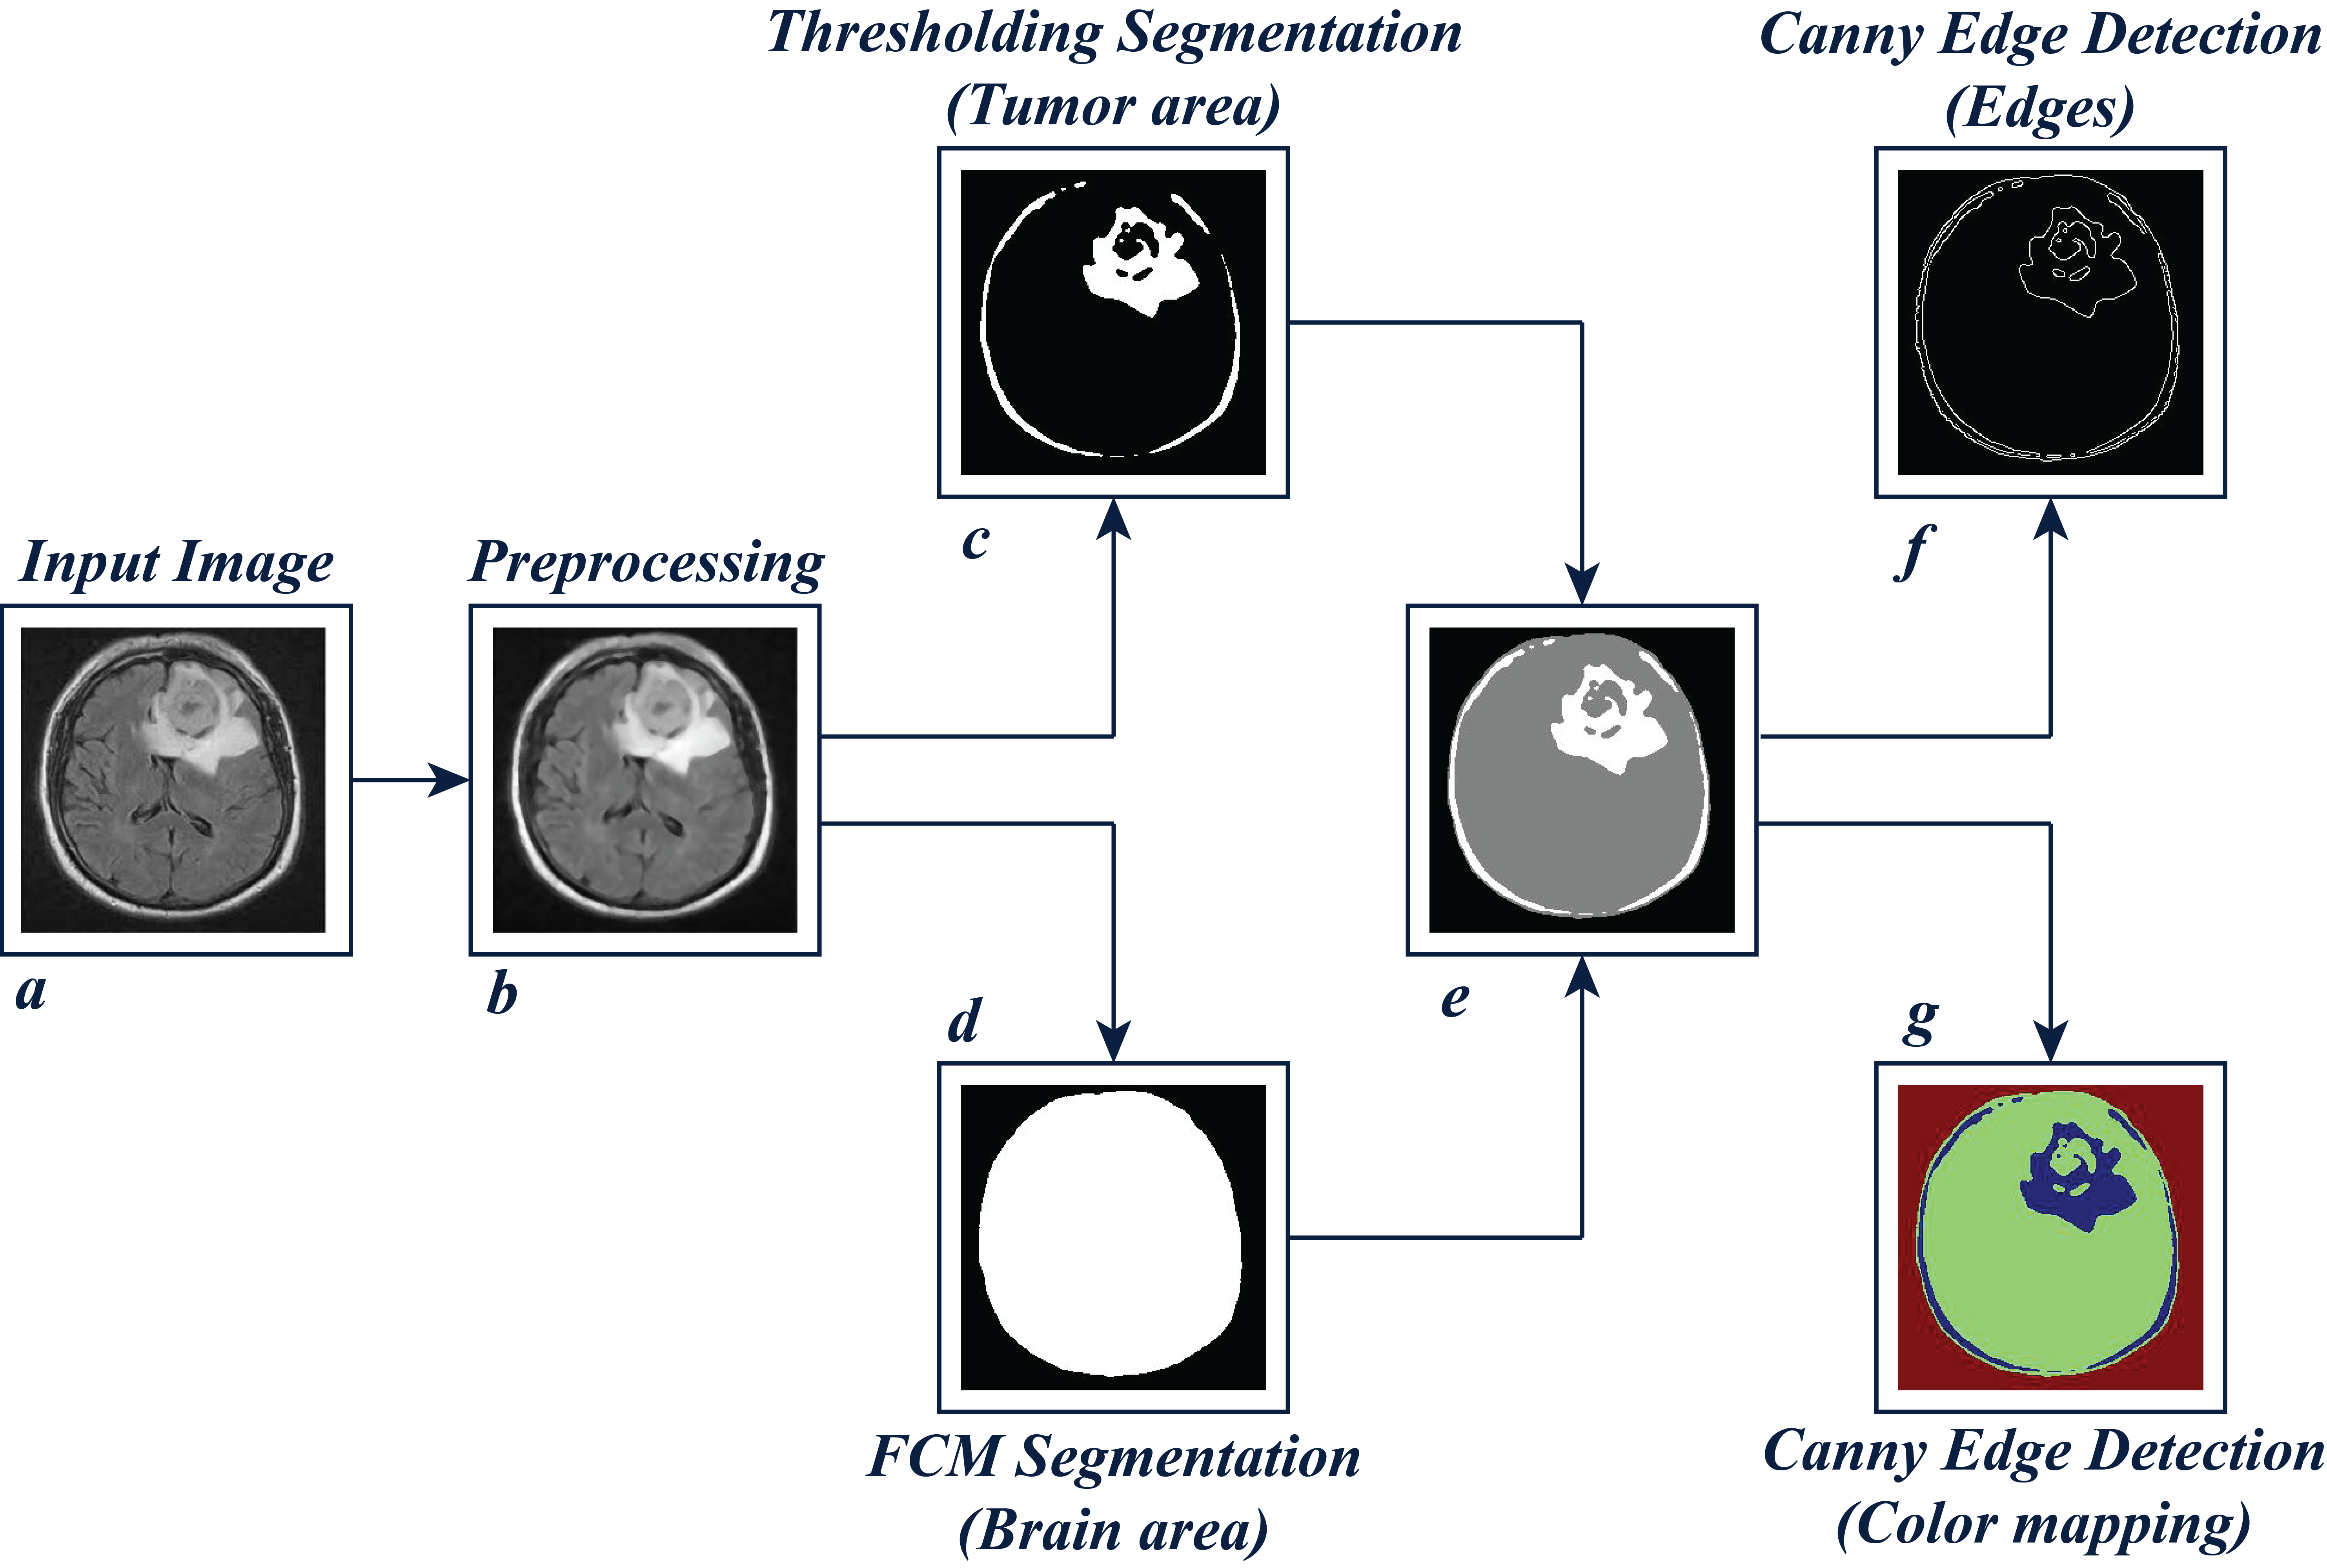
\includegraphics[width=0.9\columnwidth]{figures/Fig30.png}
	\caption{example of the system. a)input image, b)preprocessing image, c)result after thresholding, d)result after FCM clustering, e)combine both segmented images, f)final edge map, g)combined image with the color map}
	\label{fig30}
\end{figure}

This tumor segmentation system has its advantages and disadvantages. First, in cases with tumors, it has a very accurate segmentation. According to the source article, it has 97\% accuracy in detecting tumors. Also, it is simple to understand and implement due to using basic image processing and segmentation approaches. But this simplicity causes some drawbacks for this system. In MRI, tumor tissues have a similar appearance with some organs like eyes. So, usually, basic thresholding segments these normal organs as a tumor. Also, in no tumor cases, the system detects a very large brain area as the tumor.